\Exercise Donats els punts $A(1,1)$, $B=(0,-1)$ i el vector $\vec{u}=(2,4)$
\begin{llista}
  \item Calcula els vectors que van des de l'origen de coordenades cap a cadascun dels punts $A$ i $B$ (pregunta trampa...).
  \item Calcula i dibuixa $\overrightarrow{AB}$.
  \item Calcula i dibuixa $\overrightarrow{BA}$.
  \item Si $\vec{u}=\overrightarrow{AC}$, quina posició és $C$?
  \item Si $\vec{u}=\overrightarrow{CB}$, quina posició és $C$?
  \item Dóna una altres dos punts $A$ i $B$ que tinguin el mateix vector desplaçament $\overrightarrow{AB}$.
\end{llista} 

\Answer
\begin{llista}
  \item Calcula els vectors que van des de l'origen de coordenades cap a cadascun dels punts $A$ i $B$ (pregunta trampa...). El vector el trobarem substraient el punt inicial (en aquest cas $O=(0,0)$) del punt final
    \begin{itemize}
      \item \[\overrightarrow{OA}=A-O=(1,1)\]
      \item \[\overrightarrow{OB}=B-O=(0,-1)\]
    \end{itemize}
  \item Calcula i dibuixa $\overrightarrow{AB}$. 
    \[\overrightarrow{AB}=B-A=(0,-1)-(1,1)=(-1,-2)\]
    \begin{center}
      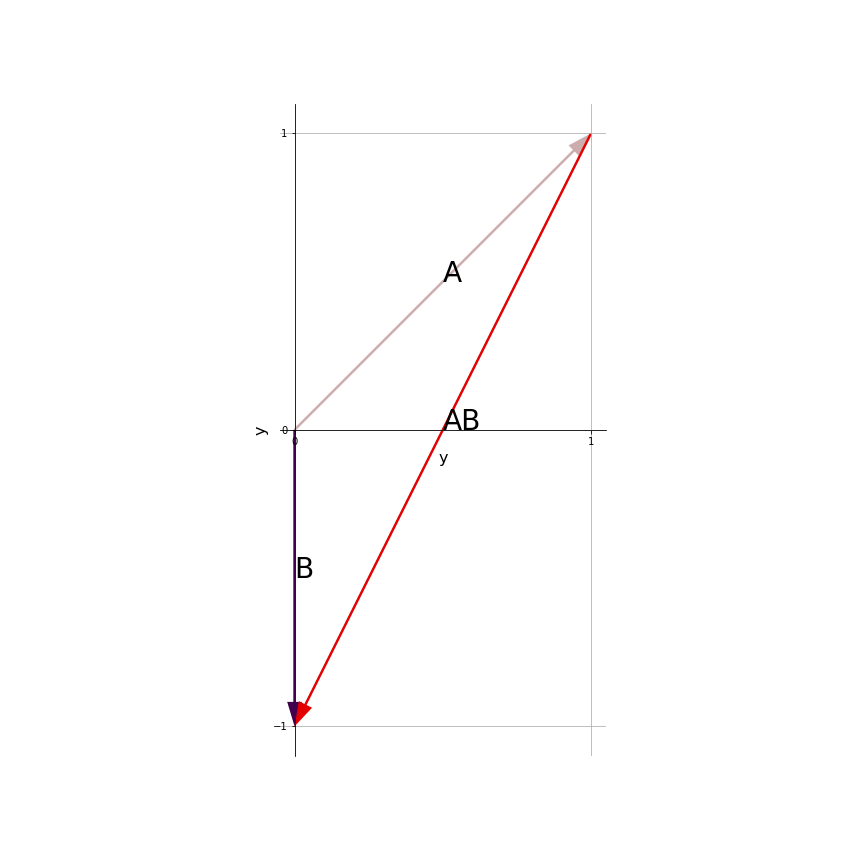
\includegraphics[scale=0.3]{vectorAB}
   \end{center}
  \item Calcula i dibuixa $\overrightarrow{BA}$.
    \[\overrightarrow{BA}=A-B=(1,1)-(0,-1)=(1,2)\]
    \begin{center}
      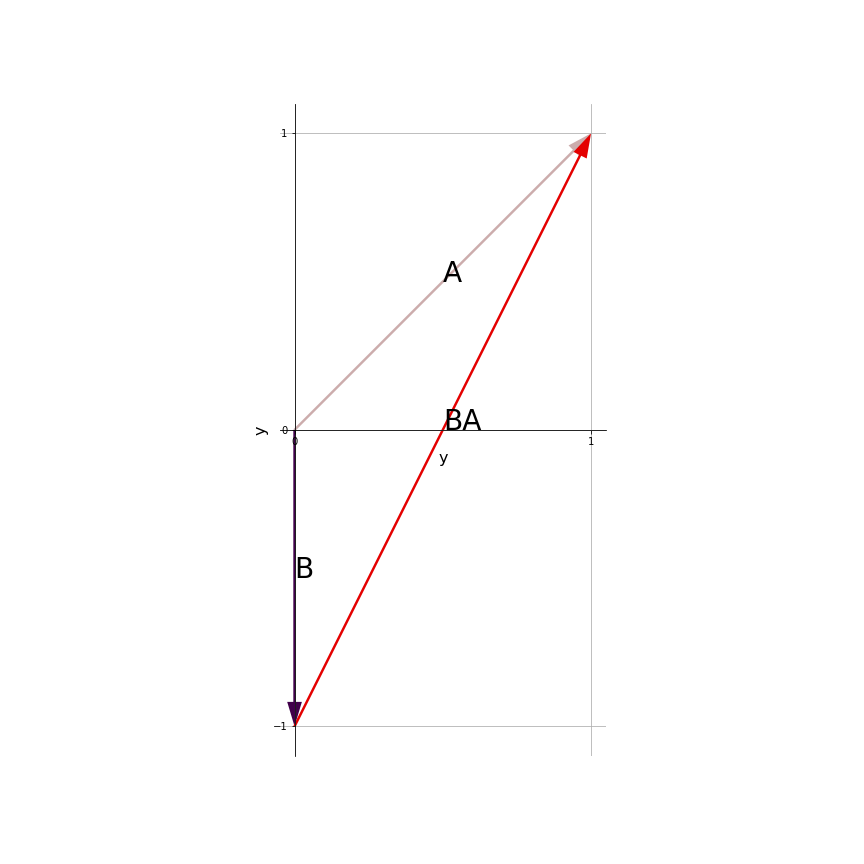
\includegraphics[scale=0.3]{vectorBA}
    \end{center}
  \item Si $\vec{u}=\overrightarrow{AC}$, quina posició és $C$?
  \[\vec{u}=\overrightarrow{AC} = C-A \Rightarrow C=A+\vec{u}=(1,1)+(2,4)=(3,5)\]
  \begin{center}
    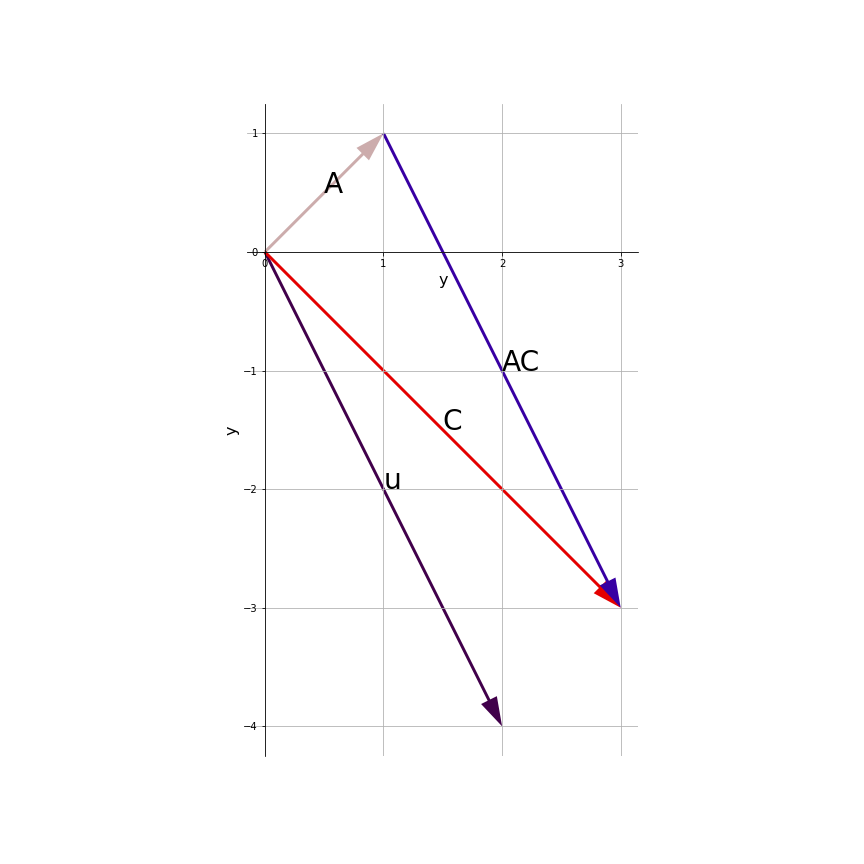
\includegraphics[scale=0.3]{vectorC1}
  \end{center}
  \item Si $\vec{u}=\overrightarrow{CB}$, quina posició és $C$?
  \item   \[\vec{u}=\overrightarrow{CB} = B-C \Rightarrow C=B-\vec{u}=(0,-1)-(1,1)=(-1,-2)\]
  \begin{center}
    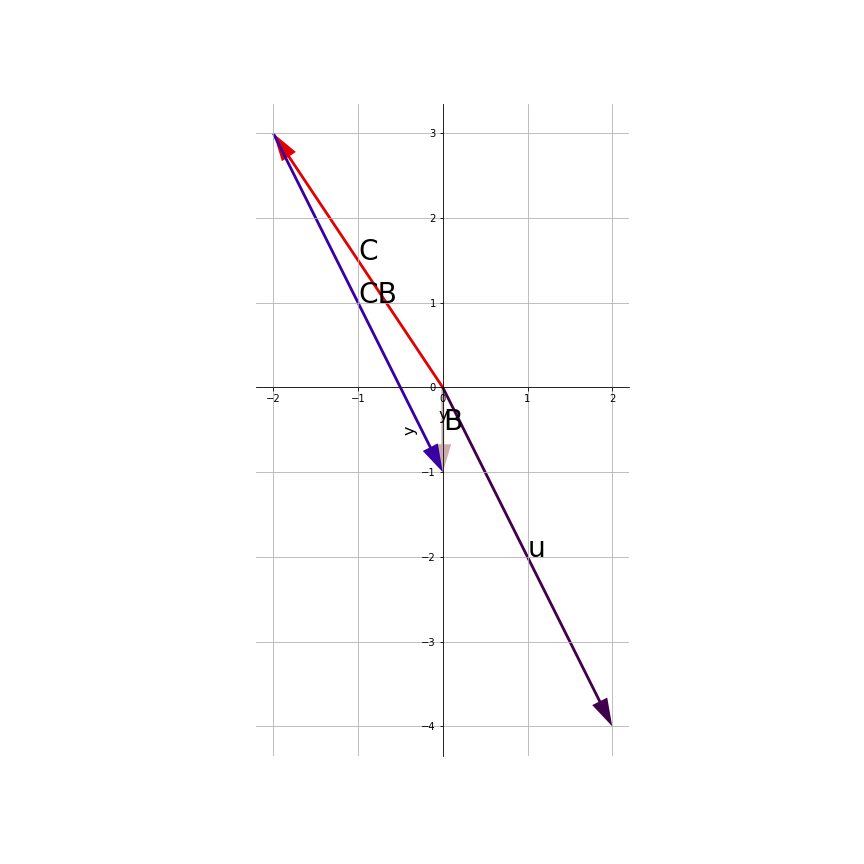
\includegraphics[scale=0.3]{vectorC2}
  \end{center}

  \item Dóna una altres dos punts $A$ i $B$ que tinguin el mateix vector desplaçament $\overrightarrow{AB}$.
  Només cal agafar un punt $D$ qualsevol i sumar-li el vector $\overrightarrow{AB}$ per trobar el punt $E$. Alguns exemples
  \begin{center}
    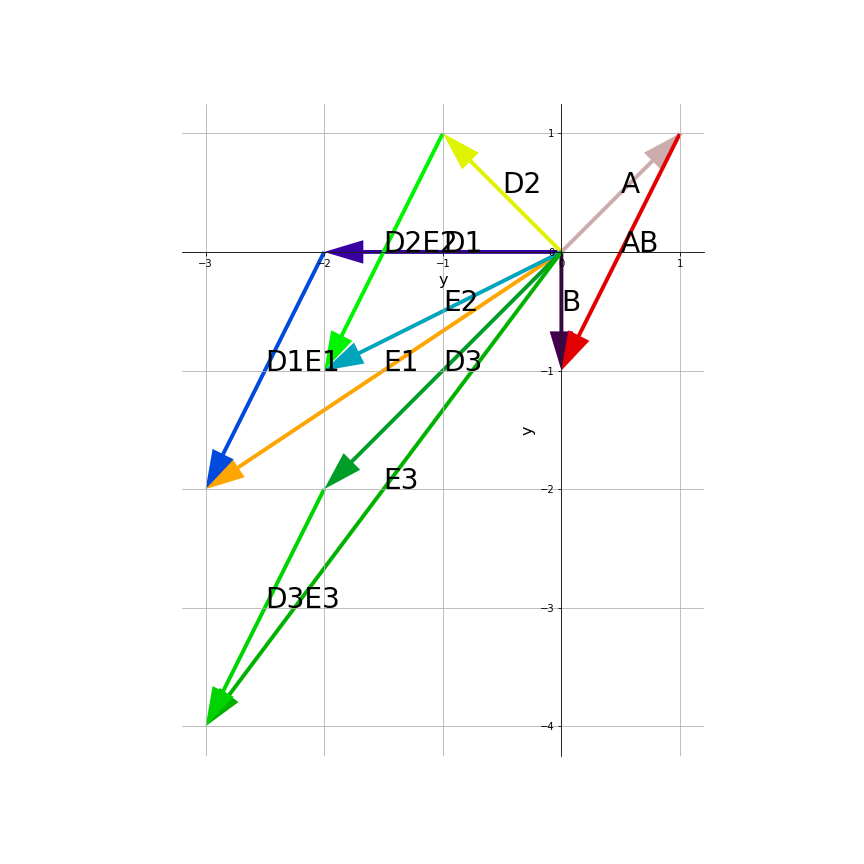
\includegraphics[scale=0.3]{vectorDE}
  \end{center}

\end{llista}
\blacksquare 